We applied our methodological framework to construct cardiometabolic comorbidity networks from UK Biobank longitudinal data. Our analysis proceeds in three stages: in Section~\ref{subsubsection:res_cosine}, we construct and validate the cardiometabolic risk-adjusted disease similarity network; in Section~\ref{subsubsection:results_conf}, we quantify confounding effects by comparing the primary risk-adjusted with the disease-only network; in Section~\ref{subsubsection:topology}, we apply GGM-based networks for sparsification and perform topological analysis. All analyses use as input embeddings extracted from the fine-tuned BioWordVec model detailed in Section~\ref{subsection:word_embedding}.

\subsection{Cardiometabolic risk-adjusted disease similarity network}\label{subsubsection:res_cosine}
The risk-adjusted cardiometabolic disease network, constructed by computing cosine similarities between disease embeddings fine-tuned on primary sequences, is shown as an adjacency matrix in Figure~\ref{fig:disease_similarity_heatmap_main_par}, with the corresponding graph visualization provided in Supplementary Figure~\ref{supp_mat:SF2}. This network constitutes our primary result, as it explicitly accounts for confounding due to shared risk-factor profiles through the joint embedding framework.

\begin{figure}[h]
    \centering
    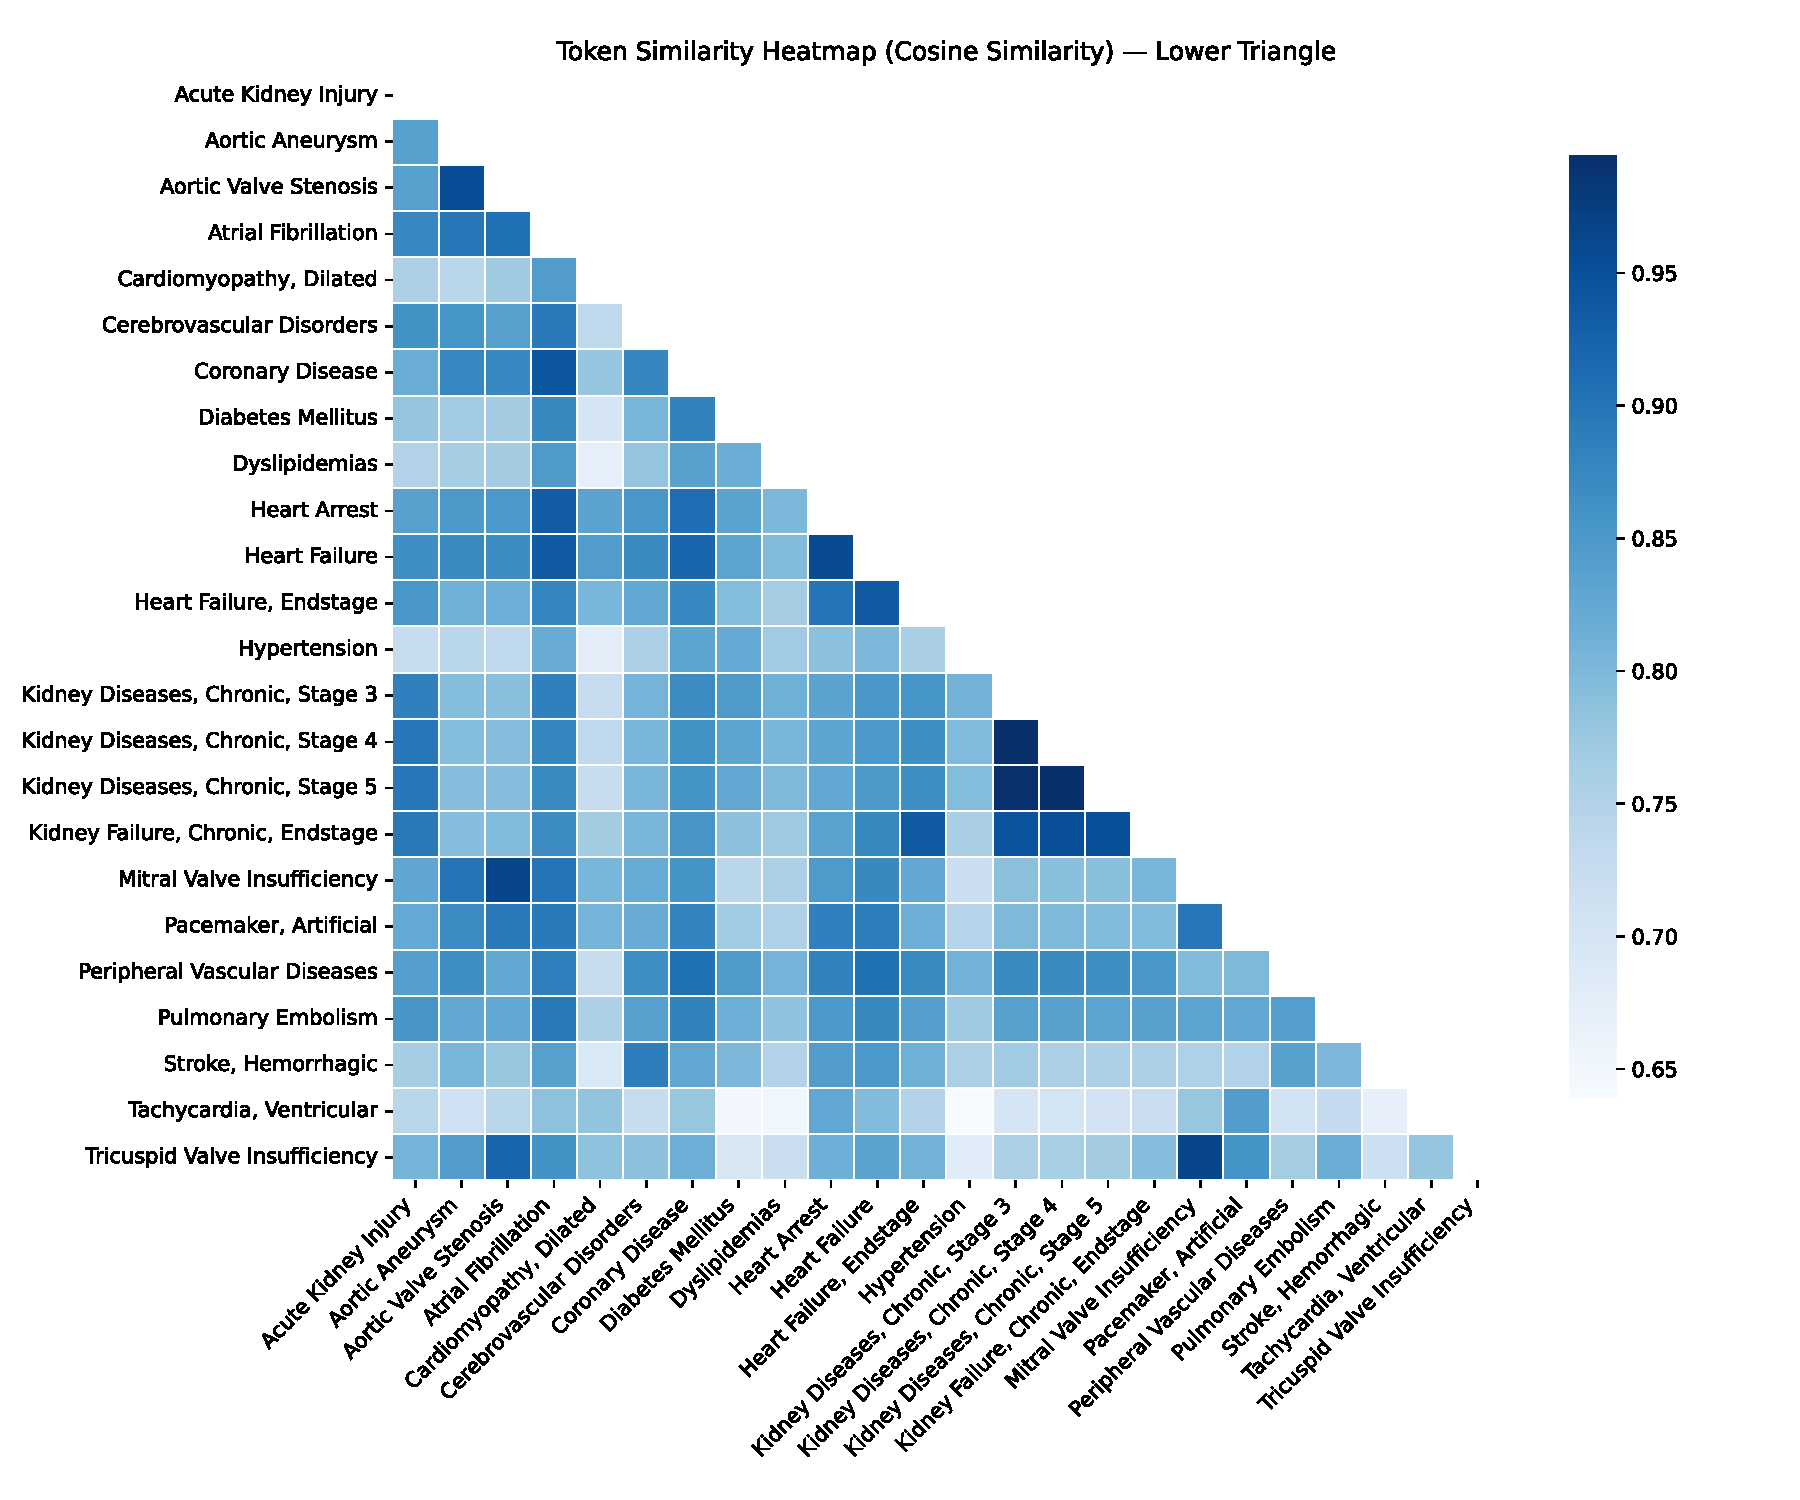
\includegraphics[width=0.9\textwidth]{Figures/disease_similarity_heatmap_main_par.pdf}
    \caption{Cosine similarity matrix for 24 cardiometabolic diseases computed from embeddings including both cardiometabolic diseases and risk factors. Darker colors indicate stronger similarities. The graph visualization is provided in Figure~\ref{supp_mat:SF2}.}
    \label{fig:disease_similarity_heatmap_main_par}
\end{figure}
The resulting adjacency matrix reveals clinically meaningful disease clusters consistent with established pathophysiological mechanisms. The chronic kidney disease (CKD) pathway emerges as a prominent domain, with strong connections between progressive renal dysfunction stages and end-stage renal disease. Acute kidney injury shows notable associations with this progression pathway, reflecting the well-documented transition from acute renal impairment to chronic dysfunction~\citet{chawla2014acute}. 
The strong similarity between heart failure and CKD stages is consistent with the cardiorenal syndrome framework, in which hemodynamic alterations, activation of the renin–angiotensin–aldosterone system, and fluid overload contribute to a bidirectional progression of disease~\citet{ronco2008cardiorenal}.
A cohesive valvular disease module emerges within the network, capturing the intrinsic dependencies among mitral, tricuspid, and aortic valve disorders. In particular, the mitral–tricuspid association is consistent with the frequent coexistence of functional tricuspid regurgitation in patients with mitral dysfunction, potentially mediated by pulmonary hypertension~(\citealp{GUERIN2019642,topilsky2018tricuspid}).
Similarly, the association between aortic stenosis and mitral valve insufficiency is well-represented, arising from left ventricular dysfunction and the systemic nature of progressive degenerative changes that simultaneously affect multiple valvular structures~\citet{genereux2013staging}. Coronary disease, atrial fibrillation, and heart failure demonstrate strong mutual associations, forming the central hub of cardiovascular multimorbidity. This triad represents the classic progression pathway where each amplifies the others through shared mechanisms, including myocardial remodelling, neurohormonal activation, and hemodynamic stress~(\citealp{santhanakrishnan2012atrial, batta2023af_cad, heusch2014cardiovascular}). Diabetes shows moderate but widespread associations across cardiovascular and renal diseases, consistent with its role as a systemic metabolic disorder affecting multiple vascular systems~\citet{usman2021interplay}. These patterns demonstrate that the risk-adjusted similarity network successfully captures established clinical relationships.

\subsection{Quantifying confounding effects through risk adjustment}\label{subsubsection:results_conf}
To validate that explicit risk factor adjustment removes confounding rather than introducing noise, we compared the risk-adjusted network presented before ($A^{(\mathcal{D+R})}$) with an unadjusted network constructed from disease-only sequences ($A^{(\mathcal{D})}$). The adjacency matrix relative to the unadjusted network is shown in~\ref{supp_mat:SF1}. Signed-difference matrix $\Delta = A^{(\mathcal{D+R})} - A^{(\mathcal{D})}$, shown in Figure~\ref{fig:disease_similarity_changes_signed}, revealed moderate but widespread changes. 
\begin{figure}[h]
    \centering
    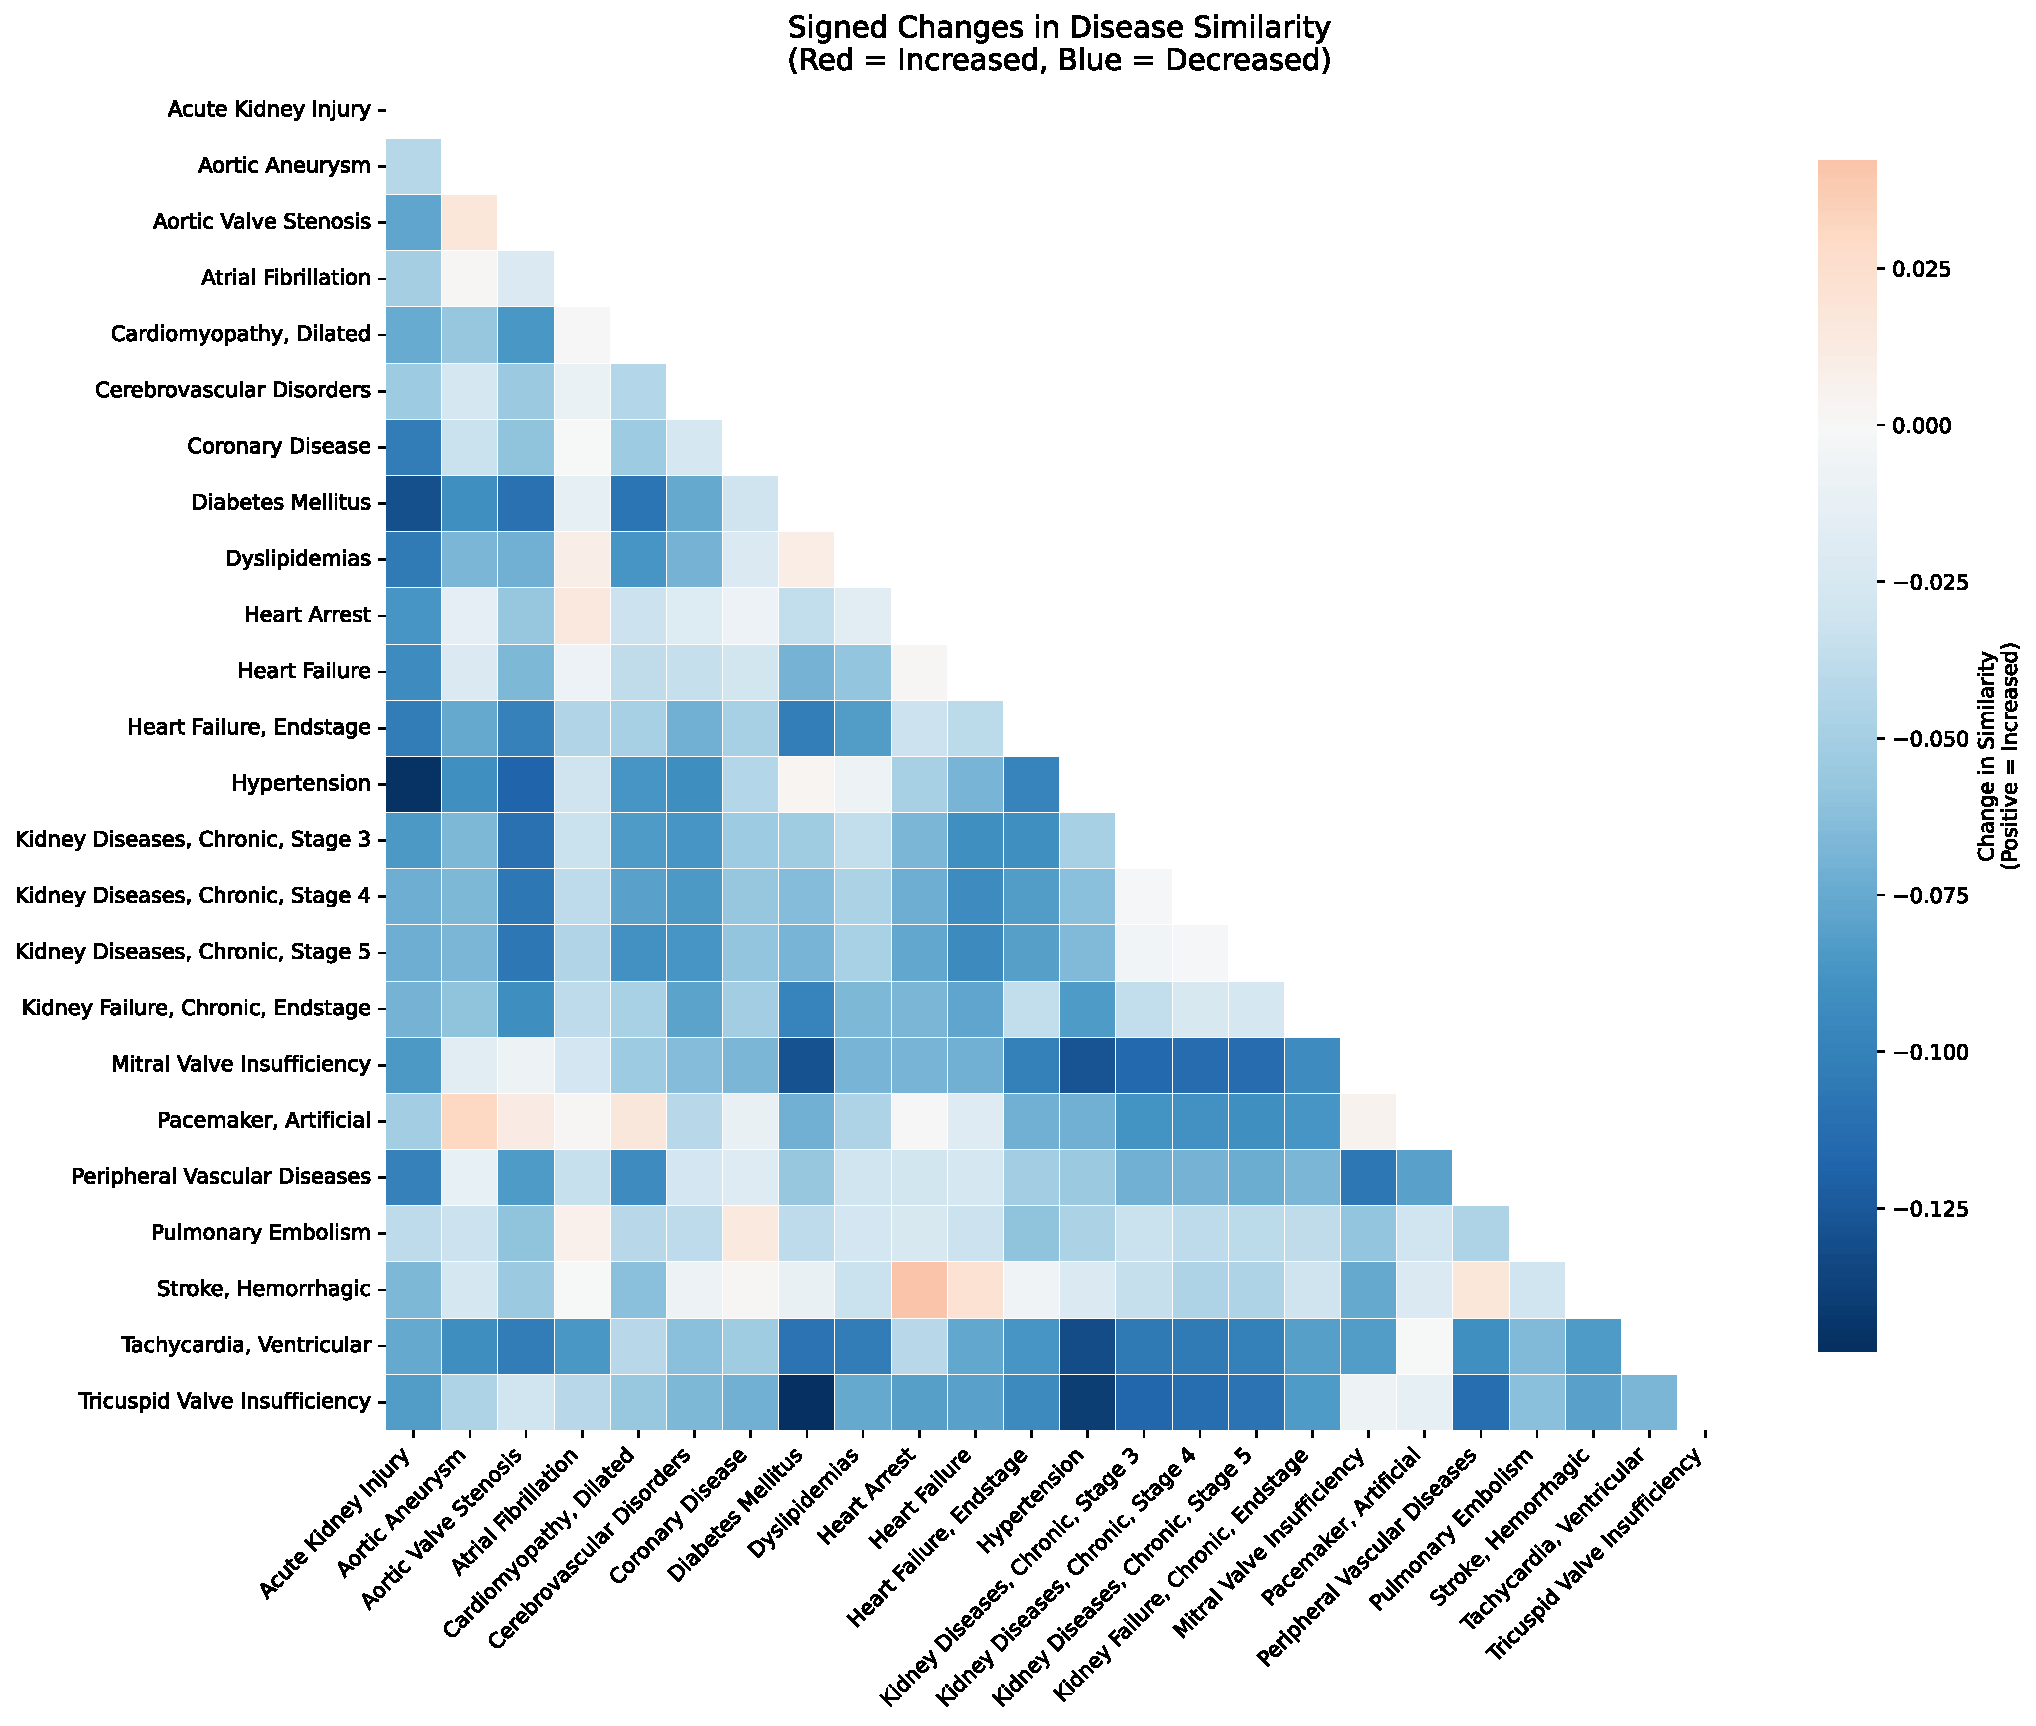
\includegraphics[width=0.9\textwidth]{Figures/disease_similarity_changes_signed.pdf}
    \caption{Signed changes in disease similarity after risk factor adjustment ($\Delta$). Blue indicates decreased similarity (confounding removal), red indicates increased similarity (unmasking true relationships).}
    \label{fig:disease_similarity_changes_signed}
\end{figure}
Global network comparison metrics are summarized in Table~\ref{tab:matrix_level_stats}. 252 of 276 disease pairs (91.3\%) exhibit decreased similarity after risk adjustment ($\Delta_{ij} < 0$), consistent with confounding removal. Only 24 pairs (8.7\%) show increased similarity ($\Delta_{ij} > 0$), potentially indicating relationships obscured by noise in the unadjusted network. The MAD across all disease pairs was moderate and the strongly negative MDC demonstrates a decreasing tendency in similarity after risk adjustment. The highly significant Wilcoxon test provides formal statistical evidence that these changes are systematic, confirming our hypothesis that shared risk factors artificially inflate disease similarities in the unadjusted network. The distribution of impact showed that 91.3\% of disease pairs experienced changes exceeding 1\%, with 12\% showing substantial changes above 10\%. Despite this evidence, Spearman correlation indicates that the fundamental ordering of disease relationships is largely preserved, suggesting that risk adjustment refines rather than fundamentally restructures the network. 

\begin{table}[h]
\centering
\begin{tabular}{lc}
\hline
\textbf{Metric} & \textbf{Value} \\
\hline
Mean Absolute Difference (MAD) & 0.060 \\
Mean Directional Change (MDC) & $-0.057$ \\
Wilcoxon signed-rank test & $p = 1.76 \times 10^{-44}$ \\
Spearman rank correlation & $\rho_S = 0.80$, $p = 3.80 \times 10^{-63}$ \\
\hline
\multicolumn{2}{l}{Impact distribution across disease pairs:} \\
\text{ } Pairs with change $> 1\%$ & 252 / 276 (91.3\%) \\
\text{ } Pairs with change $> 5\%$ & 159 / 276 (57.6\%) \\
\text{ } Pairs with change $> 10\%$ & 33 / 276 (12.0\%) \\
\hline
\end{tabular}
\caption{Matrix-level statistics comparing disease-only ($A^{(\mathcal{D})}$) versus risk-adjusted ($A^{(\mathcal{D+R})}$) similarity networks. MAD quantifies the average magnitude of change; MDC indicates systematic direction; Wilcoxon test evaluates the statistical significance of systematic change; Spearman correlation assesses structural preservation.}
\label{tab:matrix_level_stats}
\end{table}
Table~\ref{tab:top_affected_pairs_shared} reports the highly affected disease pairs (Section~\ref{subsub:conf_det} - Step 1) with the largest changes in similarity (top 5\%). All of these pairs showed a decrease in similarity. Hypertension and diabetes mellitus appear in 80\% of these most-affected pairs, particularly in association with valvular disorders and renal dysfunction. Conversely, advanced surgical interventions such as heart transplantation and artificial pacemaker implantation did not rank among the top-affected pairs, showing high stability across adjusted and unadjusted networks. To validate that these changes reflect confounding removal, we quantified shared risk factors for the most affected disease pairs (Section~\ref{subsub:conf_det} - Step 2 and 3). Highly affected disease pairs shared substantially more risk factors than lower-changed pairs (Mann-Whitney U test p-value = $2.57 \times 10^{-14}$), confirming that observed similarity decreases result from successful confounding removal rather than random variation.

\begin{table}[h]
\centering
\small
\begin{tabular}{cccc}
\hline
\textbf{Rank} & \textbf{Disease pair} & \textbf{Change} & \textbf{SharedRF} \\
\hline
1 & Tricuspid Valve Insufficiency $\leftrightarrow$ Diabetes Mellitus & -0.148 & 0.93 \\
2 & Acute Kidney Injury $\leftrightarrow$ Hypertension & -0.145 & 0.82 \\
3 & Tricuspid Valve Insufficiency $\leftrightarrow$ Hypertension & -0.140 & 0.91 \\
4 & Ventricular Tachycardia $\leftrightarrow$ Hypertension & -0.132 & 0.48 \\
5 & Acute Kidney Injury $\leftrightarrow$ Diabetes Mellitus & -0.130 & 0.86 \\
6 & Mitral Valve Insufficiency $\leftrightarrow$ Diabetes Mellitus & -0.129 & 0.83 \\
7 & Mitral Valve Insufficiency $\leftrightarrow$ Hypertension & -0.128 & 0.64 \\
8 & Hypertension $\leftrightarrow$ Aortic Valve Stenosis & -0.118 & 0.88 \\
9 & Tricuspid Valve Insufficiency $\leftrightarrow$ CKD Stage 3 & -0.117 & 0.98 \\
10 & Mitral Valve Insufficiency $\leftrightarrow$ CKD Stage 3 & -0.117 & 1.00 \\
11 & Mitral Valve Insufficiency $\leftrightarrow$ CKD Stage 4 & -0.114 & 1.00 \\
12 & Mitral Valve Insufficiency $\leftrightarrow$ CKD Stage 5 & -0.113 & 1.00 \\
13 & CKD Stage 4 $\leftrightarrow$ Tricuspid Valve Insufficiency & -0.112 & 0.99 \\
14 & Peripheral Vascular Diseases $\leftrightarrow$ Tricuspid Valve Insufficiency & -0.112 & 0.97 \\
\hline
\end{tabular}
\caption{Highly affected disease pairs (95-$th$ percentile), showing changes in similarity and SharedRF indicating the proportion of risk factors simultaneously associated (above threshold $\tau = 0.73$) with both diseases.}
\label{tab:top_affected_pairs_shared}
\end{table}

To assess the robustness of our confounding detection framework, we performed a sensitivity analysis by varying the risk factor definition threshold, $\tau$, across a range from $0.5$ to $0.9$. The results, documented in Supplementary Table~\ref{ST:shared_rf_sensitivity}, confirm the expected monotonic relationship: as $\tau$ increases, the number of risk factors associated with each disease and consequently the number of shared risk factors, decreases. At the upper bound ($\tau = 0.9$), the number of risk factors for each disease approaches zero, as this threshold significantly exceeds the mean similarity density of the risk factors' embeddings. The median achieves a balance between inclusion and exclusion of potential confounders. Notably, even as the number of individual risk factors per disease declines with higher $\tau$ values, the significance of the Mann-Whitney U test remains stable. This consistency demonstrates that our findings regarding confounding removal are robust to threshold specification. 

\subsection{Network sparsification and topology}\label{subsubsection:topology}
The sparse risk-adjusted cardiometabolic disease network, constructed using Gaussian Graphical Models, is shown as a binary adjacency matrix in Figure~\ref{fig:GGM_comorb_network_heatmap} with the corresponding graph visualization provided in Supplementary Figure~\ref{supp_mat:SF3}. Compared to the fully connected cosine similarity network, the GGM network exhibits only half of the edge density but the majority of pathophysiological relationships identified in Section~\ref{subsubsection:res_cosine}.
\begin{figure}[h]
    \centering
    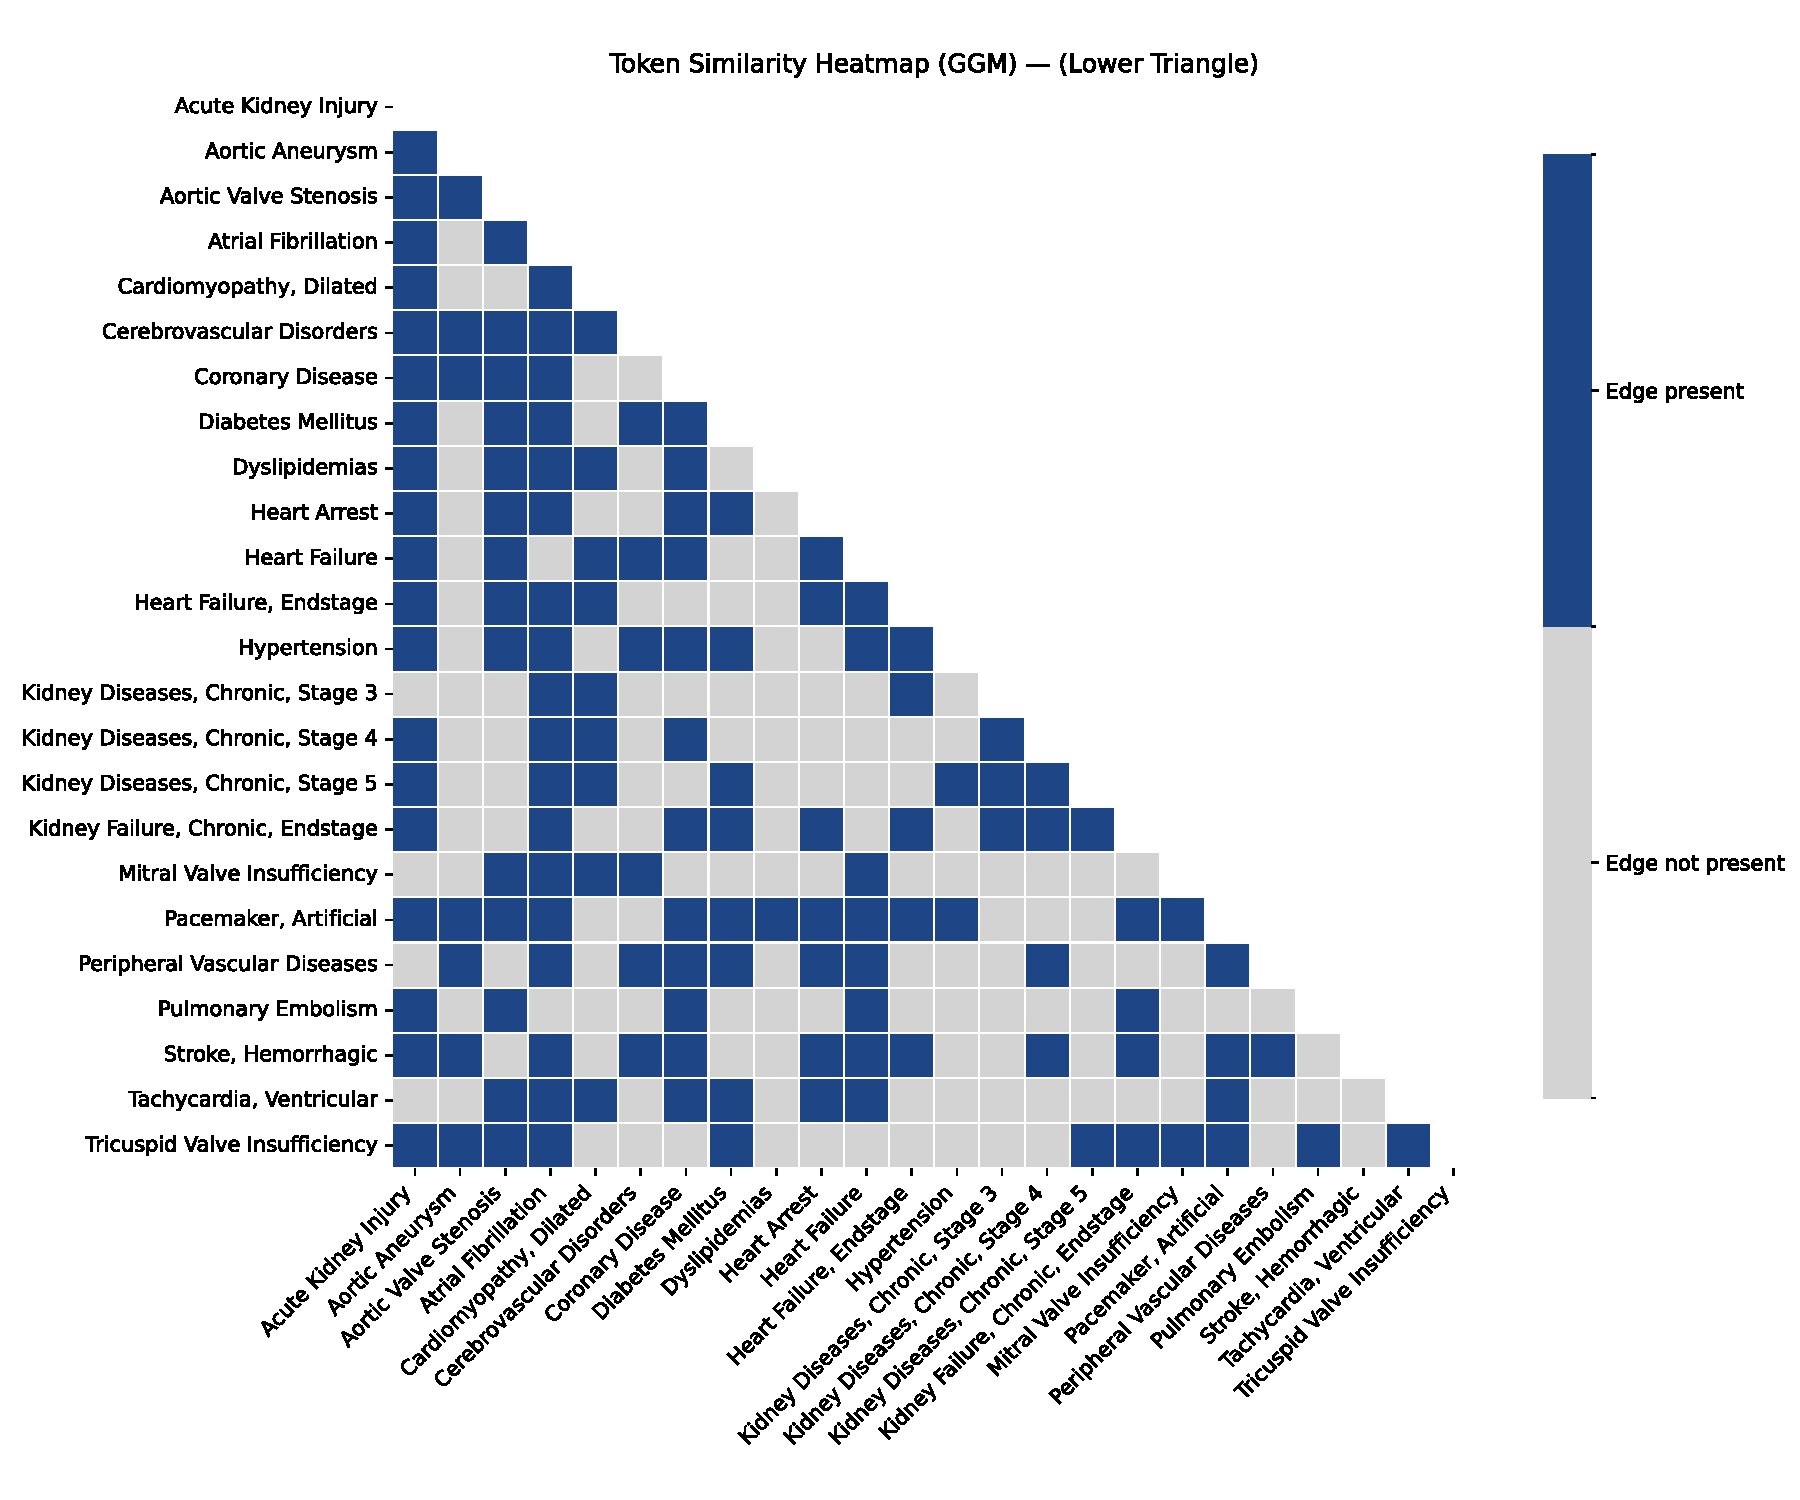
\includegraphics[width=0.9\textwidth]{Figures/disease_GGM_heatmap_main_par_binary.pdf}
    \caption{Cardiometabolic disease matrix estimated via Gaussian Graphical Lasso Regression computed from embeddings including both cardiometabolic diseases and risk factors. The graph representation is provided in Supplementary Figure~\ref{supp_mat:SF3}.}
    \label{fig:GGM_comorb_network_heatmap}
\end{figure}
To identify key pathological determinants within the network, we quantified node importance through degree and betweenness centrality measures. The results for the most central nodes are summarized in Table~\ref{tab:top5_centrality}, with comprehensive metrics for all phenotypes provided in Supplementary Table~\ref{ST:centrality}. Atrial fibrillation emerges as the primary hub with the highest degree and betweenness centrality, reflecting both its epidemiological prevalence and its critical position bridging multiple pathophysiological domains, including thromboembolism, heart failure, and cerebrovascular disease. Acute kidney injury ranks second in both centrality measures, underscoring its role as a key mediator within the cardiorenal syndrome pathway. The high betweenness centrality indicates that acute kidney injury facilitates the transition from acute cardiovascular insults to chronic renal dysfunction, connecting distinct pathological states. The elevated betweenness of the artificial pacemaker node, despite representing an intervention rather than a disease, reflects its function as a bridging state between primary arrhythmias, structural heart disease, and heart failure. Coronary disease occupies a central tier, linking ischemic pathophysiology to systemic metabolic disorders such as diabetes and peripheral vascular disease. While heart failure exhibits concentrated associations within cardiovascular and cardiorenal modules, the strong betweenness of aortic valve stenosis highlights its role in connecting valvular pathology to large-vessel disease. 

\begin{table}[h]
\centering
\small
\begin{tabular}{ccc}
\hline
\textbf{Rank} &\textbf{Degree} & \textbf{Betweeness} \\
\hline
1 & Atrial Fibrillation & Atrial Fibrillation \\
2 & Acute Kidney Injury & Acute Kidney Injury \\
3 & Artificial Pacemaker & Artificial Pacemaker \\
4 & Aortic Valve Stenosis / Coronary Disease & Coronary Disease \\
5 & Heart Failure & Aortic Valve Stenosis \\
\hline
\end{tabular}
\caption{Top 5 diseases ranked by betweenness and degree centrality in the GGM network. Details on centrality for other disease are provided in Supplementary Table~\ref{ST:centrality}.}
\label{tab:top5_centrality}
\end{table}

The application of the fast greedy modularity optimization algorithm to the GGM-derived network identified a latent community structure consisting of three distinct disease modules. This partition, shown in Figure~\ref{fig:community_detection}, reflects the primary biological domains of cardiometabolic pathology. The first module (cardiorenal-metabolic, color-coded blue) captures the continuum of heart-kidney failure, integrating progressive renal dysfunction with metabolic disorders. The second module (primary cardiovascular, color-coded pink) aggregates conditions originating from cardiac structural damage and electrical dysfunction. The third module (large vessel and cerebrovascular, color-coded green) shares the etiology of systemic vasculopathy, linking aortic pathology with peripheral and cerebral vascular disease. Notably, nodes such as acute kidney injury and atrial fibrillation were identified as inter-community bridges, maintaining high betweenness centrality while connecting the cardiorenal-metabolic and primary cardiovascular clusters.
 
\begin{figure}[h]
    \centering
    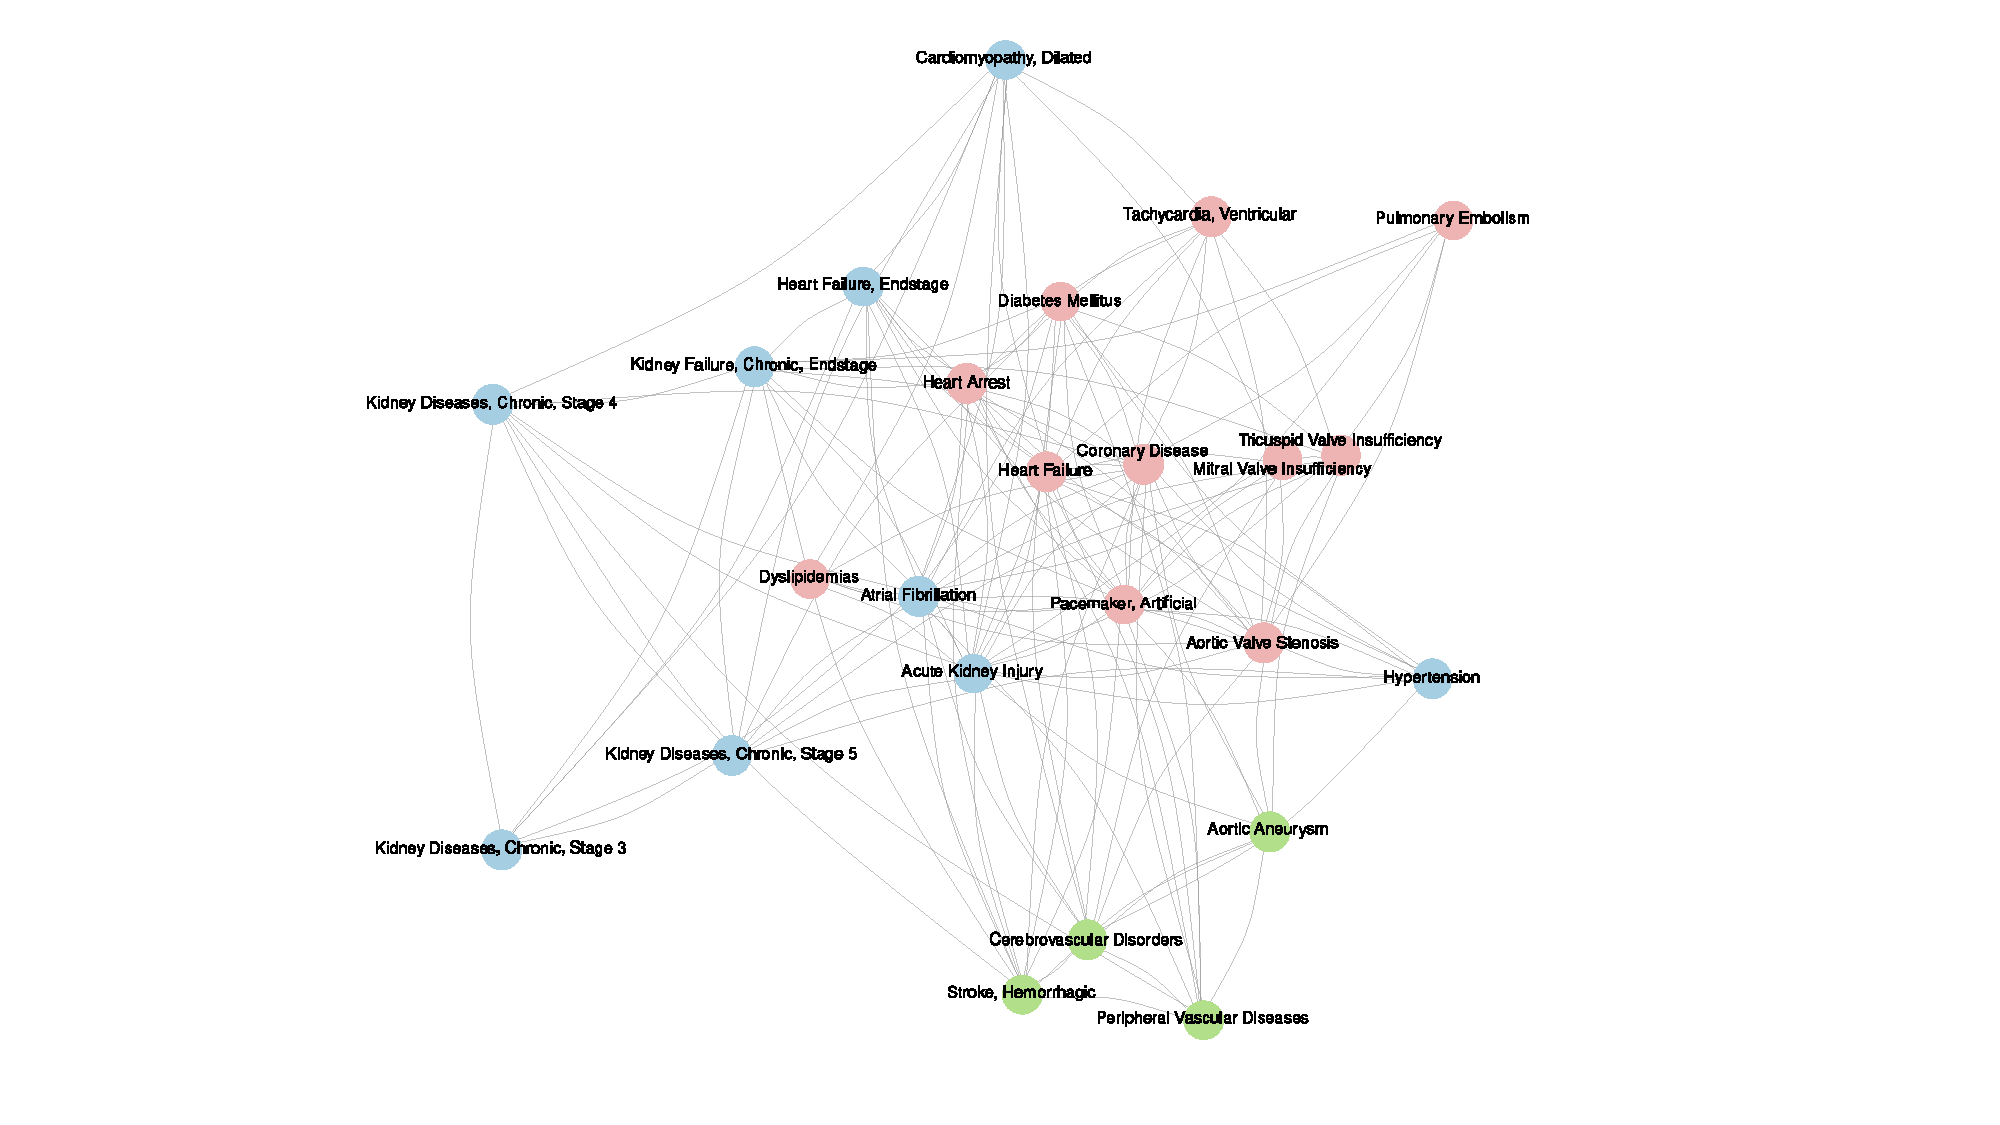
\includegraphics[width=0.95\textwidth]{Figures/community_detected.pdf}
    \caption{Community structure of the cardiometabolic disease network identified via fast greedy modularity optimization. Node colors indicate community membership: \textit{blue} = cardiorenal-metabolic module, \textit{pink} = primary cardiovascular module, \textit{green} = large vessel and cerebrovascular module.}
    \label{fig:community_detection}
\end{figure}

